The requirements in this document follow a hierarchical structure where indented requirements represent data or quality requirements that are connected to their parent functional requirement. This structure helps show the relationships between functional requirements and their associated quality attributes or data specifications.

For example, a functional requirement like \textbf{HeatmapSearch} may have indented quality requirements such as \textbf{HeatmapPerformance} that specify performance criteria for that feature.

\subsection{Heatmap Visualization}

\begin{tabular}{|p{.95\textwidth}|}
    \hline
    \textbf{Task:  Find cheap trip destination using heatmap}\\
    \hline
    Subtasks:
    \begin{enumerate}
        \item Input origin / allow location data
        \item Input flight dates
        \item Navigate heatmap
        \item Select area
        \item Select show details for flight
        \item Get referred to airline
    \end{enumerate}\\
    \hline
    Variants:
    \begin{enumerate}
        \item[1a.] User types in origin airport
        \item[1b.] User uses device location data for origin
    \end{enumerate}\\
    \hline
\end{tabular}

\textbf{HeatmapSearch}: The system shall display a heatmap that visually represents flight prices for various destinations, with the lowest available prices highlighted using colors, engaging users in the search process. See an example in \autoref{fig:mockup2}.
    \begin{quote}
        \textbf{HeatmapPerformance}: The heatmap should update dynamically within 3 seconds of data input or changes such as price range. \\ \\
        Monitor UI logs to confirm rendering completion time after changes to input data.
    \end{quote}
    \begin{quote}
        \textbf{HeatmapVisibility}: The heatmap shall be responsive and maintain readability on screen sizes ranging from 320px (mobile) to 1920px (desktop). It shall use a color gradient that ensures a minimum contrast ratio of 4.5:1 (WCAG AA) for text labels and distinguishable color differences between price categories. See \autoref{fig:mockup1} and \autoref{fig:mockup2}. Note the examples are only prototypes and are not final.
    \end{quote}
\textbf{DateRangeMap}: Travellers and Travel Agencies can change the dates for which the map shows data. Domain-level control for flight search customization.
    \begin{quote}
        \textbf{DateChangeResults}: The map should reflect date changes in under 2 seconds without requiring a full reload. \\ \\
        Monitor UI logs to confirm rendering completion time after date modifications.
    \end{quote}
\begin{quote}
    \textbf{FlexibleRangeMap}: The system should support flexible date ranges spanning at least 30 days for price comparisons. \\ \\
    Test by selecting a range of 30-60 days, verifying the system returns results across all days without errors.
\end{quote}
\textbf{ListFlightsFromMap}: Travellers and Travel Agencies can see a text list of destinations with the lowest flight prices shown on map. Product-level display of destinations based on search.
    \begin{quote}
        \textbf{TextListsShown}:Destination lists should be updated in real-time when new flight deals become available. \\ \\
        Insert a new deal in the back-end or get deal from airlines API and verify update propagation within milliseconds.
    \end{quote}
\textbf{AirportSelection}: Travellers and Travel Agencies can select airports from the heatmap. Product-level feature allowing interactive selection.
\begin{quote}
    \textbf{FastAirportSelection}: Selected airports should be highlighted instantly and search results updated in under 2 seconds. \\ \\ 
    Measure UI update times via browser dev tools or performance logs.
\end{quote}

\subsection{User Security}
\textbf{LawCompliance}:The system should comply with general data protection regulations (GDPR). Domain-level requirement ensuring user data privacy.
\begin{quote}
    \textbf{GDPRCompliance}: Perform a data protection regulations (GDPR) audit to ensure compliance with data protection regulations. \\ \\
    Document and address any issues found during the audit.
\end{quote}
\textbf{SecureDataEncryption}: User data should be encrypted both in transit and at rest. Domain-level security requirement.
\begin{quote}
    \textbf{DataEncryptionCheck}: Ensure that all user data is encrypted using secure protocols and stored securely. \\ \\
    Perform security audits and penetration tests to verify encryption and storage mechanisms.
\end{quote}

\subsection{Flight Search}

\begin{tabular}{|p{.95\textwidth}|}
    \hline
    \textbf{Task: Find cheap flight}\\
    \hline
    Purpose: Find cheap flight to general area\\
    \hline
    Input parameters:
    \begin{itemize}
        \item Origin
        \item Destination
        \item Dates
    \end{itemize}\\
    \hline
    Display options:
    \begin{itemize}
        \item Heatmap
        \item List
        \item Filter
        \item Date sliders
    \end{itemize}\\
    \hline
\end{tabular}

\textbf{SearchCheapFlights}: Travellers and Travel Agencies can find destinations with low flight prices when providing a departure city and dates. Search results shall be ranked by price in ascending order, ensuring the most cost-effective options are prominently displayed. Goal-level requirement defining a key system function.
\begin{quote}
    \textbf{FastSearchResults}: Search results should be displayed within 2 seconds for queries that include a departure city, and travel dates, retrieving data for up to \_ available flights.\\ \\ 
    Tested by generating random inputs and measuring response time using automated performance testing tools, logging response times for 1000+ random queries.
\end{quote}
\textbf{ListCheapFlights}: The system shall present a structured list of available flights to a specified destination, sorted by price in ascending order. Product-level feature for displaying search results.
\begin{quote}
    \textbf{TextListSupport}: The list should support sorting by price, duration, and airline, with sorting applied in under 1 second.\\ \\ 
    Use UI performance tests to time sorting actions on datasets of varying sizes for example destinations with a lot of flights or destinations with less flights.
\end{quote}
\textbf{SearchCheapDestinations}: Travellers and Travel Agencies can find flights to a given destination. Domain requirement focusing on the flight search feature.
\begin{quote}
    \textbf{FastPriceDisplay}: The system shall retrieve and display flight prices within 2 seconds for search requests that include a departure city, and travel dates, processing up to \_ flight options per request.\\ \\
    Execute automated tests simulating 1000+ searches and log the response time until results are fully rendered. Primarily same as \textit{FastSearchResults}.
\end{quote}
\textbf{DateRangeSearch}: Travellers and Travel Agencies should be able to provide a range of possible dates for their flight search making the service more flexible and appealing to a wider range of users. Domain-level functionality supporting flexible searches, in flight search feature.
\begin{quote}
    \textbf{DateRangeCheck}: The system should support flexible date ranges spanning at least 30 days for price comparisons. \\ \\
    Test by selecting a range of 30-60 days, verifying the system returns results across all days without errors.
\end{quote}
\textbf{GeolocationService}: Travellers can have their device provide their current location. Domain-level feature leveraging geolocation services.
\begin{quote}
    \textbf{GeoLocationCheck}:Location detection should be completed in under 3 seconds with at least 95\% accuracy.\\ \\
    Use GPS data from 50 ore more test cases across different devices and measure accuracy based on expected vs. detected locations.
\end{quote}
\textbf{ShowFlights}: Traveller can click through to ticket booking page for shown flights. Product-level requirement enabling ticket purchase.
    \begin{quote}
        \textbf{CorrectNavigation}: Clicking a flight should navigate to the booking page within 1 second and fill in relevant details from users account. \\ \\
        Use automated UI testing to time redirection and fill in data according to users account.
    \end{quote}
\textbf{SaveFavoriteCity}:A signed-in traveller can save favorite cities. Product-level feature for personalization.
\begin{quote}
    \textbf{FavoriteCityFetching}: Favorite cities should be stored in under 5 seconds and retrievable in under 1 second. \\ \\
    Save favorite cities and time retrieval speed via API performance monitoring.
\end{quote}

\subsection{User Experience}
\textbf{UsabilityScore}: The ease of use of the product shall be tested and must achieve a System Usability Score (SUS) of at least 70 points, indicating acceptable usability.
\begin{quote}
    \textbf{SUSTesting}: Conduct usability tests with a sample group of users and calculate the SUS score. \\ \\
    Ensure the average score meets or exceeds 70 points.
\end{quote}

\textbf{AccessibilityCompliance}: The accessibility of the product shall be tested and must comply with WCAG 2.1 standards.
\begin{quote}
    \textbf{WCAGTesting}: Perform accessibility audits using automated tools and manual testing to ensure compliance with WCAG 2.1 standards. \\ \\
    Document and address any issues found during testing.
\end{quote}

\textbf{RegularUserFeedback}: The system shall regularly prompt users for feedback. Product-level feature that aims to gather user insights and improve customer satisfaction by understanding user experiences and expectations. 
\begin{quote}
    \textbf{FeedbackCheck}: After \_ hours of use, the system shall prompt the user with the question "What do you think about EasyTrip?" and a rating scale. 
\end{quote}

\subsection{Account Management \& Personalization}
\textbf{AccountCreation}: Travellers should be able to create accounts. Product-level requirement for account management.
\begin{quote}
    \textbf{AccountData - Data dictionary}: Product-level requirement: \\\textbf{Class}: User\\
    The user is a Traveller or Travel Agency who has a user account in the product.
    
    \textbf{Examples}:
    1. A traveller who has a user account.
    2. A travel agency who uses their user account to search flights.
    
    \textbf{Attributes}:
    \begin{enumerate}
        \item \textbf{email}:      Text, 320 chars
        The user's email address. This email address is used for communication with the user outside the product.
        \item \textbf{name}:       Text, 50 chars
                The name of the traveller or travel agency using the account.
        \item \textbf{newsletter}: Boolean
        Whether the user wants mass email's from the product or not.
        \item \textbf{city}:       Text, 35 chars
        The city the user's default origin is set to. This is the standard origin used when performing searches for the user.
    \end{enumerate}    
\end{quote}

\begin{quote}
    \textbf{AccountData - Virtual window}: Product-level requirement described using a data dictionary: \\\textbf{Class}: \begin{longtable}{|p{3cm}|p{9cm}|}
        \hline
        \rowcolor{headergray}
        \textbf{Field} & \textbf{Value} \\ \hline
        \textbf{Email} & exampleJohn@gmail.com \\ \hline
        \textbf{Name} & John Doe \\ \hline
        \textbf{Utskick} & True \hspace{1em} False \\ \hline
        \textbf{City} & New York \\ \hline
    \end{longtable}
\end{quote}

\textbf{EmailConfirmation}: The ownership of travellers' email addresses should be confirmed. Domain requirement ensuring valid accounts.
    \begin{quote}
        \textbf{ConfirmationCheck}: Email verification links should be sent within 5 seconds and expire after 24 hours. \\ \\
        Log email dispatch times in the system and verify expiration behavior after 24 hours.
    \end{quote}
\textbf{CreateAccountEmail}: Travellers should be able to create accounts with email addresses and passwords. Productlevel authentication requirement.  
    \begin{quote}
        \textbf{}: The registration process should take no longer than 15 seconds, including email verification. \\ \\
        Automate user sign-ups and measure time from form submission to receiving the verification email.
    \end{quote}
\textbf{EmailChange}: Travellers should be able to change their email address. Product-level account management feature.
\begin{quote}
    \textbf{EmailChangeConfirmationPerformance}: Changes to email addresses should be confirmed within 10 seconds via a verification email.\\ \\
    Track the end-to-end time from submission of email change request to email receipt.
\end{quote}
\textbf{ChangePassword}:Travellers should be able to change their passwords. Product-level security feature.
    \begin{quote}
        \textbf{CheckChangePassword}:Password changes should be effective after 5 seconds and require strong passwords (at least 8 characters, uppercase, lowercase, number, symbol). \\ \\
        Verify enforcement of password complexity rules and Ensure old credentials become invalid 5 seconds after post-update.
    \end{quote}
\textbf{PasswordReset}: Travellers should be able to reset their password if they have forgotten it. Product-level usability requirement.
\begin{quote}
    \textbf{FastPasswordReset}: Reset emails should be sent within 10 seconds and expire after 30 minutes. \\ \\
    Log email dispatch times and attempt password resets after 30 minutes to confirm expiration.
\end{quote}
\textbf{MarketingConsent}: Travellers should be asked about receiving marketing emails during account creation. This consent should be editable in real-time in the Account management section. The system should log consent preferences for auditing purposes. Domain-level requirement ensuring compliance with marketing preferences.
\begin{quote}
    \textbf{EmailPreferenceCheck}:Marketing email preferences should be configurable and updated in real-time. \\ \\ 
    Toggle marketing settings in the Account management section and verify backend logs reflect changes within 5 seconds.
\end{quote}

\subsection{System Performance}
\textbf{StatisticsReport}: Product manager and IT maintenance can request a statistics report containing number of searches and response times. Goal-level requirement for system analytics.
\begin{quote}
    \textbf{FastStatisticsReport}: Reports should be generated in under 10 seconds for a dataset covering the last 6 months. \\ \\
    Execute test report requests and measure query execution and rendering time.
\end{quote}
\textbf{AnonymizedData}: User data should be anonymized for analytics. 
\begin{quote}
    \textbf{AnonymizedCheck}: Ensure that all personally identifiable information (PII) is removed or obfuscated before generating reports. Verify through data audits and compliance checks. \\ \\
\end{quote}
\textbf{DynamicResourceAllocation}: The system should allocate computing resources (for example memory and CPU), dynamically based on load to ensure scalability. Goal-level requirement for system scalability.
\begin{quote}
    \textbf{ResourceAllocationCheck}: The system should scale up to handle \_ concurrent users without slowdown. \\ \\
    Simulate \_ concurrent users with load-testing tools and measure system response time. For example AWS.
\end{quote}
\textbf{UptimeGuarantee}: The system should have an uptime of at least 99.9\%. Goal-level requirement for system reliability.
\begin{quote}
    \textbf{UptimeMonitoring}: Monitor system uptime and ensure it meets the 99.9\% requirement. \\ \\
    Use uptime monitoring tools to track system availability over time.
\end{quote}
\textbf{AutoFailoverMechanism}: The system should have an automatic failover mechanism. The system should automatically switch to a backup server in case of a failure. Goal-level requirement for system reliability.
\begin{quote}
    \textbf{FailoverTesting}: Simulate a system failure and verify that the failover mechanism is triggered within 5 seconds. \\ \\
    Use automated tests to simulate system failures and measure failover time.
\end{quote}
\textbf{APIIntegrationSupport}: The system should support integration with external APIs. Goal-level requirement for system extensibility.
\begin{quote}
    \textbf{APIIntegrationCheck}: Ensure that the system can integrate with at least the necessary external APIs without performance degradation. \\ \\
    Test system performance with and without API integrations to measure impact.
\end{quote}

\subsubsection{Data Model}
\textbf{DataModel}: The product level data requirements are represented through a E/R diagram in \autoref{fig:data-model}, it shows the data used \\ \\
for the flight searches and the user accounts in the system.

\begin{figure}[H]
    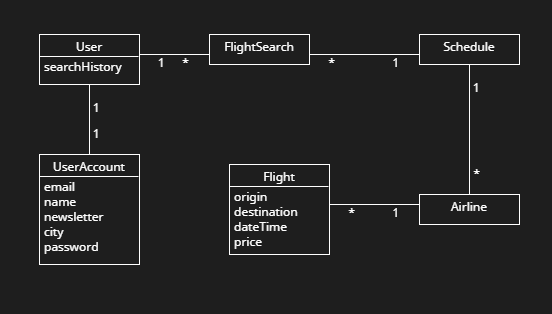
\includegraphics[width=1\textwidth]{resources/dataRelations.PNG}
    \caption{Entity/Relationship data model}
    \label{fig:data-model}
\end{figure}

\subsection{Others}
\textbf{MultipleTicketPrices}: Travellers and Travel Agencies can see prices for multiple tickets. Product-level requirement enabling comparison of ticket prices.
\begin{quote}
    \textbf{FastMultiTicketPrices}: The system should allow searching for up to 10 passengers simultaneously without affecting response time. Test by searching for 10 tickets and verifying that all prices are displayed without errors.\\ \\
     Compare response times of searches with 1 vs. 10 passengers under normal and peak loads.
\end{quote}
\textbf{MultiFlightTrips}: Travellers and Travel Agencies can find prices of multi-flight trips. Product-level requirement for multi-leg trip pricing.
    \begin{quote}
        \textbf{PriceRetrieval}:The system should retrieve multi-flight prices in less than 5 seconds, considering layovers and airlines. \\ \\ 
        Run tests for complex multi-leg searches, logging response times for different scenarios.
    \end{quote}
\textbf{MarketingChannels}: Marketers can send marketing emails to travelers who have explicitly opted in through the account management settings. Product-level marketing function.
\begin{quote}
    \textbf{CheckMarketing}: Marketing emails should be delivered to 95\% of recipients within 1 minute of sending. \\ \\
    Track email delivery timestamps for mass campaigns and compute success rate over time.
\end{quote}
\textbf{B2BFindFlights}: Travel agencies can find flights on behalf of clients. Goal-level requirement supporting B2B services.
\begin{quote}
    \textbf{B2BMultipleSearch}: Travel agency accounts should support handling at least 50 concurrent searches without slowdown. \\ \\ 
Simulate 50+ concurrent users with load-testing tools for example JMeter and measure system response time.
\end{quote}
\textbf{AdProviders}: The product shall display ads from Ad Providers.

%TODO ADD DESCRIPTION TO FOLLOWING PART
\begin{table}[h]
    \centering
    \renewcommand{\arraystretch}{1.5}
    \begin{tabular}{|l|c|c|c|c|c|}
        \hline
        & \textbf{Critical} & \textbf{Important} & \textbf{As usual} & \textbf{Unimportant} & \textbf{Ignore} \\
        \hline
        \textbf{Operation} & & & & & \\
        Integrity/security & & & x & & \\
        Correctness & & & x & & \\
        Reliability/availability & 1 & & & & \\
        Usability & 3 & & & & \\
        Efficiency & & 2 & & & \\
        \hline
        \textbf{Revision} & & & & & \\
        Maintainability & & & x & & \\
        Testability & & & x & & \\
        Flexibility & & & x & & \\
        \hline
        \textbf{Transition} & & & & & \\
        Portability & & & & x & \\
        Interoperability & & 4 & & 4 & \\
        Reusability & & & & & x \\
        Installability & & 5 & & & 5 \\
        \hline
    \end{tabular}
    \caption{Software Quality Characteristics}
    \label{tab:quality_characteristics}
\end{table}

\subsection*{Explanations}
\begin{enumerate}
    \item It is critical that the system is always available since it can be used by anyone across the world, meaning we have the potential to gain customers at any time of the day. If availability is below 99\%, the company loses money, and key stakeholders, such as airlines, are negatively impacted.
    \item If the system cannot filter or return proper search results quickly, users may grow impatient and leave for a competitor.
    \item The system must be easy to navigate and use since our customer base includes anyone willing to travel. Users will have a wide range of experience using websites. Since our differentiation lies in ease of learning we deem it critical that the usability and ease of learning needs to meet our quality requirements.
    \item The system is not required to interact with other systems like file transfers or specific hardware. However, some components need to cooperate with external systems, such as our ad provider or direct links to airlines for flight booking.
    \item Since the system is web-based on computer workstations, installation is unnecessary. However, for the mobile version, an app must be installed, which should be easy to download from platforms like the App Store or Google Play.
\end{enumerate}

\newpage
\begin{figure}[h]
    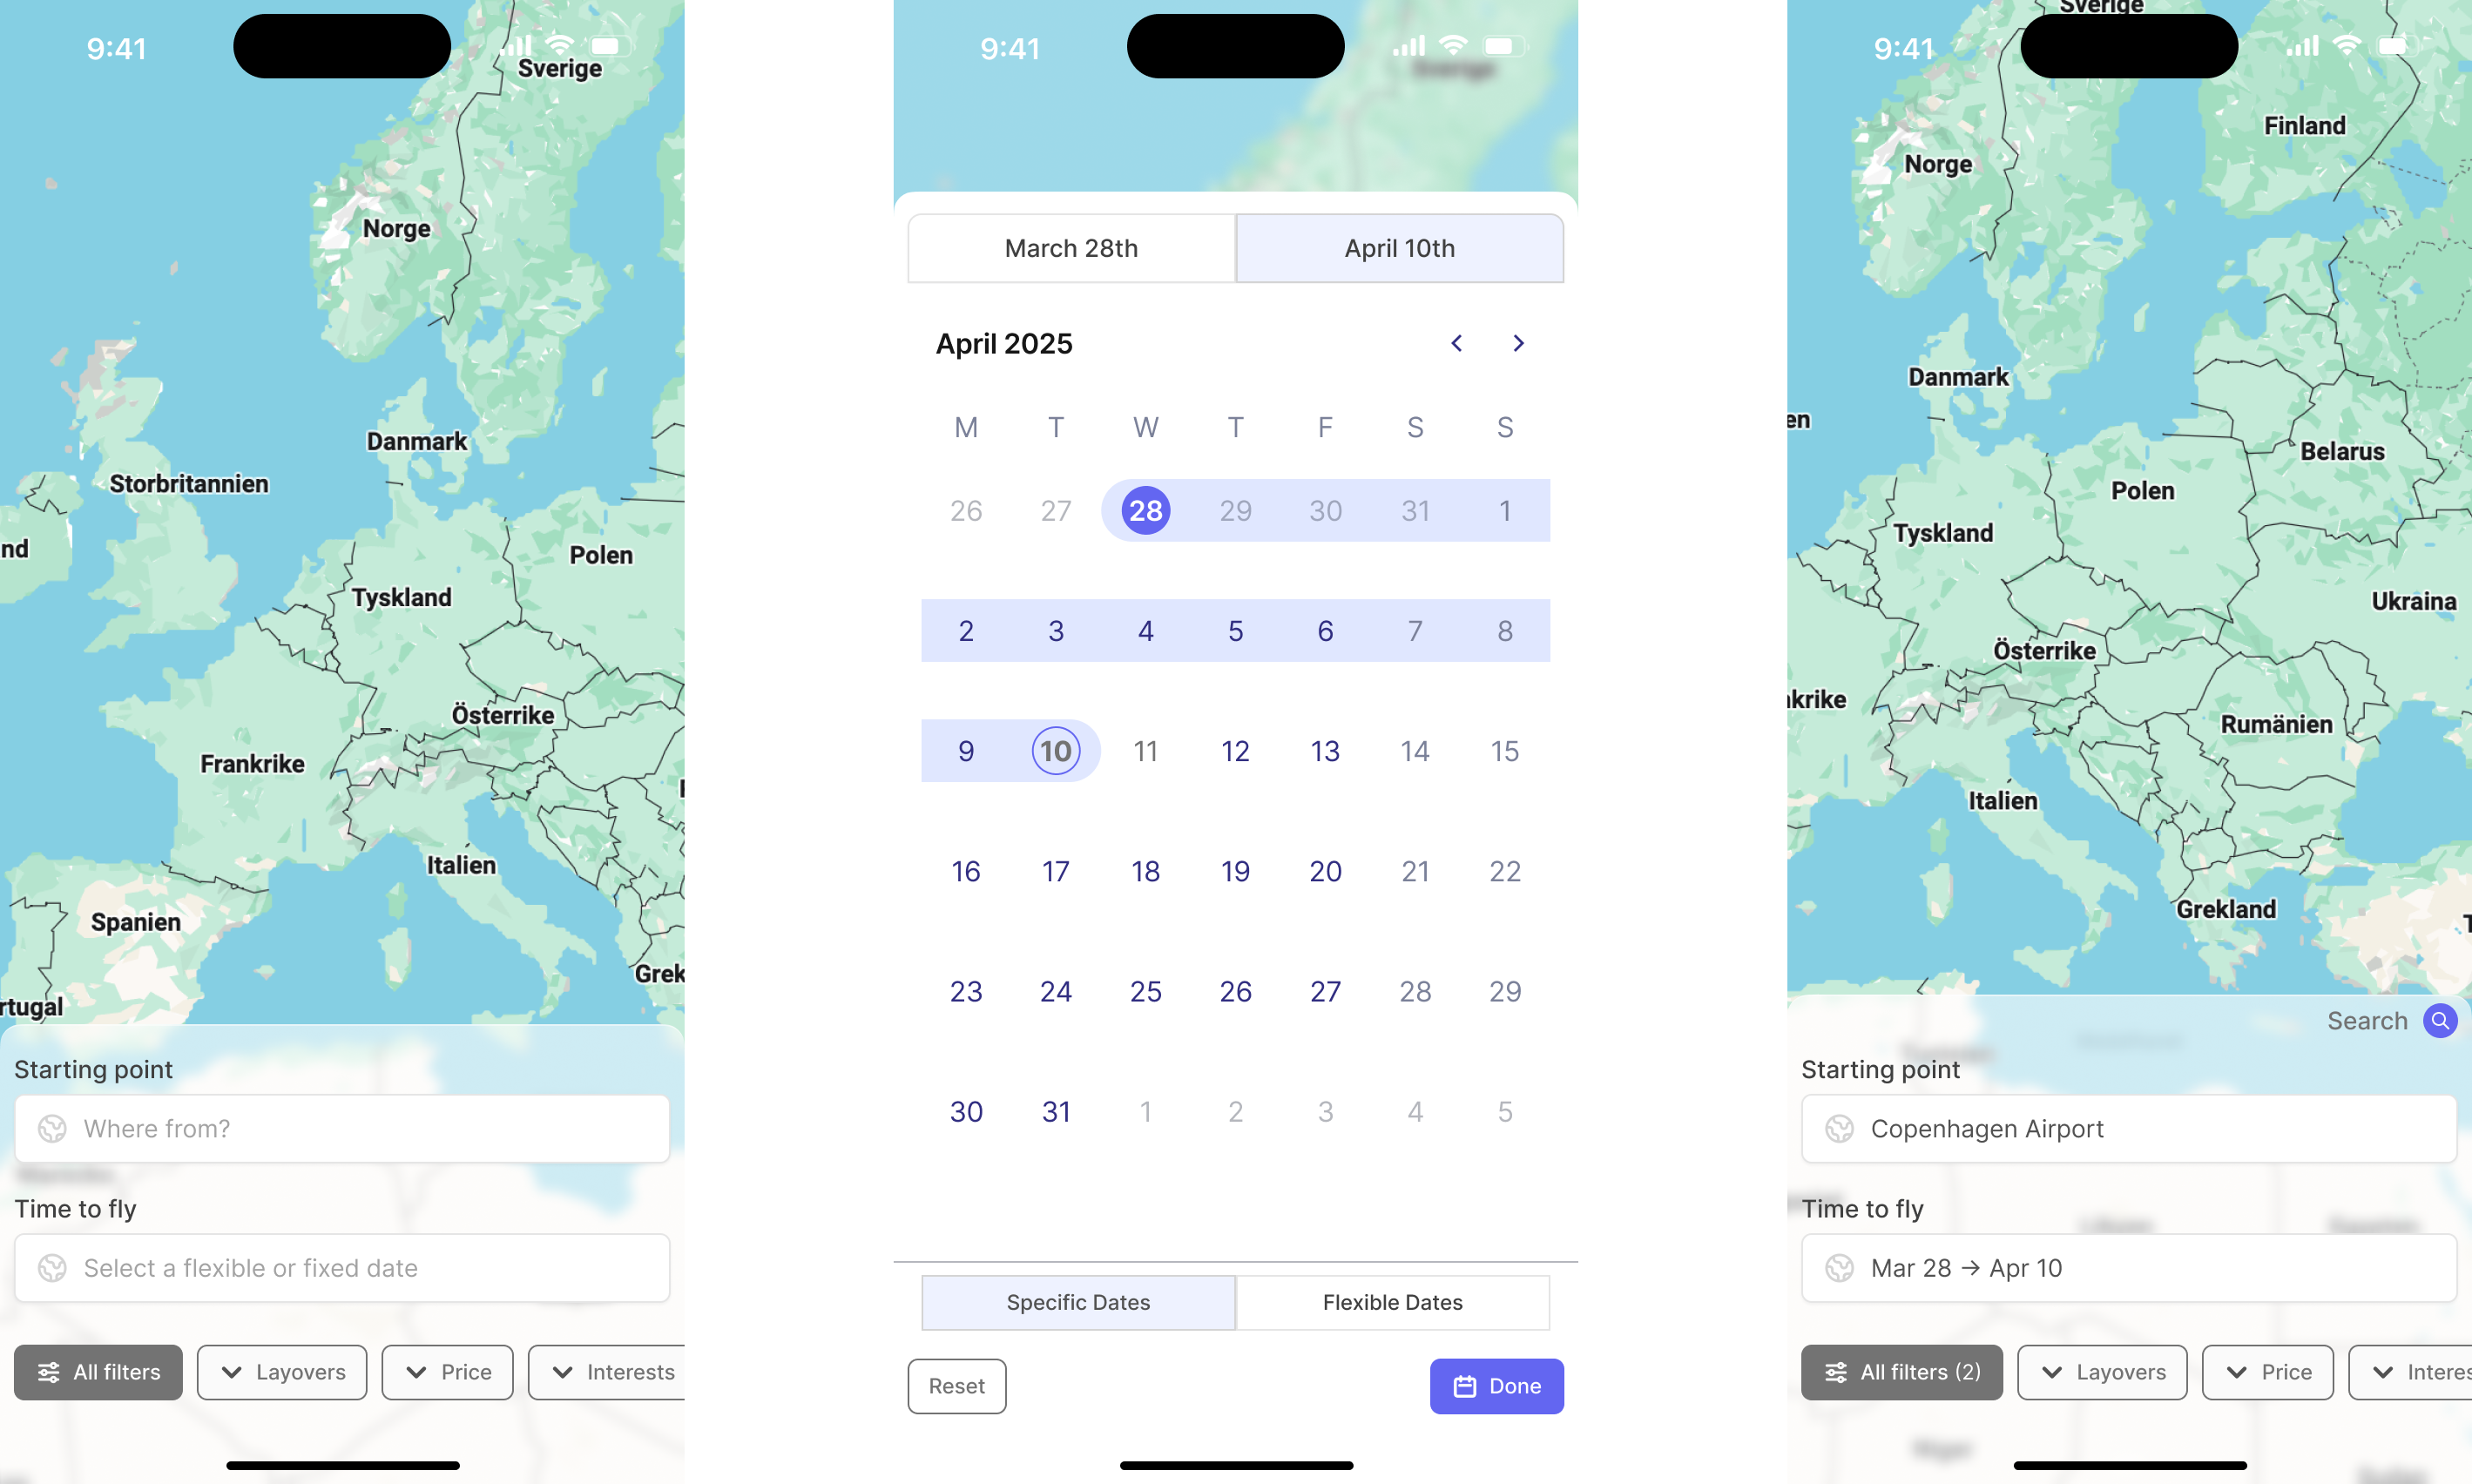
\includegraphics[width=.89\textwidth]{resources/mockup1.png}
    \caption{User interface showing the search page, dynamic date picker and filters.}
    \label{fig:mockup1}
\end{figure}

\begin{figure}[h]
    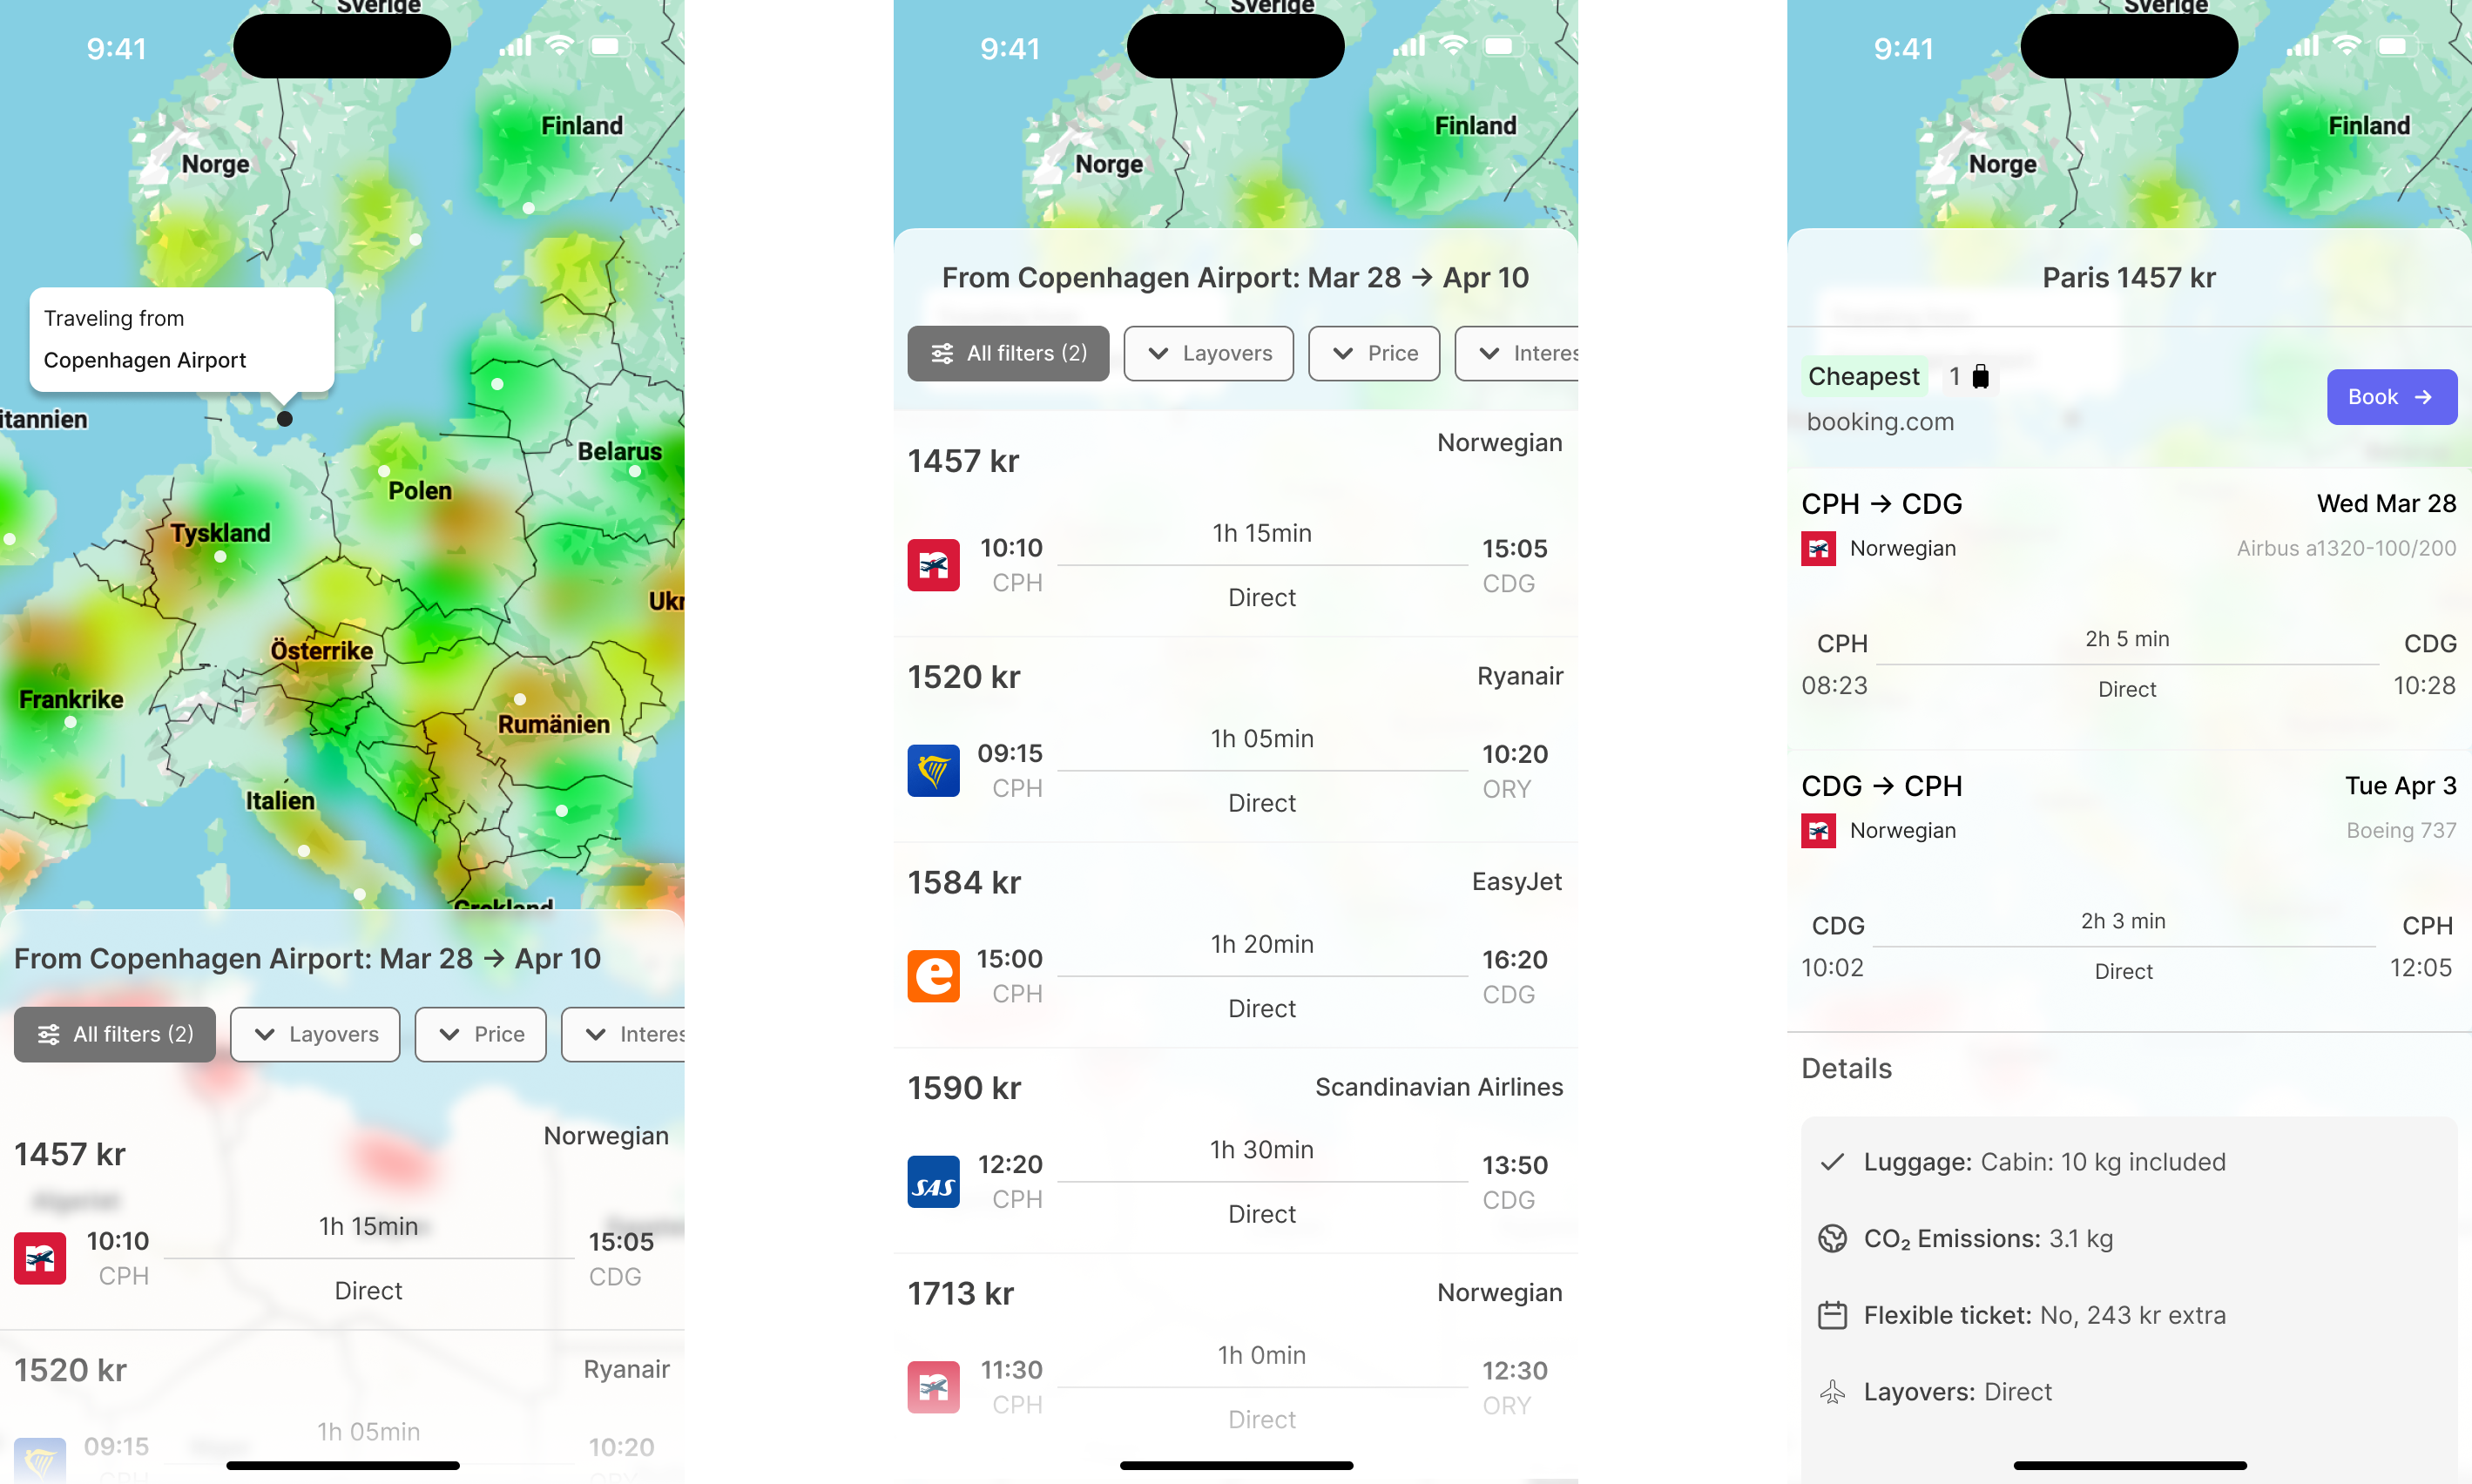
\includegraphics[width=.89\textwidth]{resources/mockup2.png}
    \caption{User interface showing the search results page with a list of flights and a heatmap.}
    \label{fig:mockup2}
\end{figure}

\newpage
